\subsection{Least Squares Approximation}

It should not be surprising to hear that many problems do not have a
perfect solution, and in these cases the objective is always to try to
do the best possible. For example what does one do if there are no
solutions to a system of linear equations $A\vect{x}=\vect{b}$? It
turns out that what we do is find $\vect{x}$ such that $A\vect{x}$ is
as close to $\vect{b}$ as possible. A very important technique that
follows from orthogonal projections is that of the least square
\index{least square approximation} approximation, and allows us to do
exactly that.

We begin with a lemma. 

Recall that we can form the image of an $m \times n$ matrix $A$ by
$\func{im}\left( A\right) = = \left\{ A\vect{x} : \vect{x} \in
\mathbb{R}^n \right\}$. Rephrasing Theorem \ref{thm:orthproj} using
the subspace $W=\func{im}\left( A\right)$  gives the
equivalence of an orthogonality condition with a minimization
condition.\index{orthogonality and minimization} The following picture
illustrates this orthogonality condition and geometric meaning of this
theorem.

\begin{center}
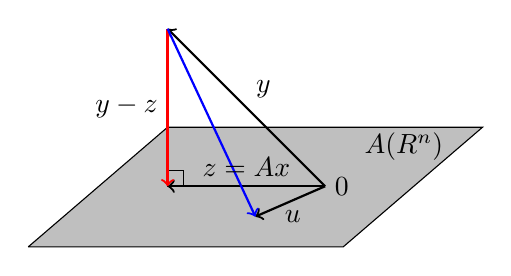
\begin{tikzpicture}
\draw[fill=lightgray](-3,0,2)--(-2,0.75,0)--(2,0.75,0)--(1,0,2)--(-3,0,2);
\draw(-2,0,0) rectangle (-1.8, 0.2,0);
\draw[thick,->](0,0,0)--(-2,0,0);
\draw[thick,->](0,0,0)--(-2,2,0);
\draw[red,thick,->](-2,2,0)--(-2,0,0);
\draw[thick,->](0,0,0)--(-0.5,0,1);
\draw[blue, thick, ->](-2,2,0)--(-0.5,0,1);
\node[right] at (0,0,0){$0$};
\node[above] at (-1,0,0){$\vect{z}=A\vect{x}$};
\node[above right] at (-1,1,0){$\vect{y}$};
\node[left] at (-2,1,0){$\vect{y}-\vect{z}$};
\node[right] at (-0.25,0,1){$\vect{u}$};
\node at (1,0.5,0){$A(\mathbb{R}^n)$};
\end{tikzpicture}
\end{center}

\begin{theorem}{Existence of Minimizers}{existenceminimizerhs}\label{existenceminimizerhs}
Let $\vect{y}\in \mathbb{R}^{m}$ and let $A$ be an $m\times n$ matrix.

Choose $\vect{z}\in W= \func{im}\left( A\right)$ given by $\vect{z} =
\func{proj}_{W}\left( \vect{y}\right)$, and let $\vect{x} \in \mathbb{R}^{n}$ such that $\vect{z}=A\vect{x}$.

Then
\begin{enumerate}
\item $\vect{y} - A\vect{x} \in W^{\perp}$
\item $\vectlength \vect{y} - A\vect{x} \vectlength < \vectlength \vect{y} - \vect{u} \vectlength$ for all $\vect{u} \neq \vect{z} \in W$
\end{enumerate}
\end{theorem}

We note a simple but useful observation.

\begin{lemma}{Transpose and Dot Product}{transposeanddotprod}
Let $A$ be an $m\times n$ matrix. Then 
\begin{equation*}
A\vect{x} \dotprod \vect{y} = \vect{x}\dotprod A^T\vect{y} 
\end{equation*}
\end{lemma}

\begin{proof}
This follows from the definitions:
\[ A\vect{x} \dotprod \vect{y}=\sum_{i,j}a_{ij}x_{j} y_{i}
=\sum_{i,j}x_{j} a_{ji} y_{i}= \vect{x} \dotprod A^T\vect{y}
\] \end{proof}

The next corollary gives the technique of least squares.

\begin{corollary}{Least Squares and Normal Equation}{normalEquation}
A specific value of $\vect{x}$ which solves the problem of Theorem 
\ref{thm:existenceminimizerhs} is obtained by solving the equation
\begin{equation*}
A^TA\vect{x}=A^T\vect{y}
\end{equation*}
Furthermore, there always exists a solution to this system of equations.
\end{corollary}

\begin{proof} 
For $\vect{x}$ the minimizer of Theorem \ref{thm:existenceminimizerhs}, $\left(
\vect{y}-A\vect{x}\right) \dotprod A \vect{u} =0$ for all $\vect{u} \in \mathbb{R}^{n}$ and from
Lemma \ref{lem:transposeanddotprod}, this is the same as saying
\begin{equation*}
A^T\left( \vect{y}-A\vect{x}\right) \dotprod \vect{u}=0
\end{equation*}
for all $u \in \mathbb{R}^{n}.$ This implies 
\begin{equation*}
A^T\vect{y}-A^TA\vect{x}=\vect{0}.
\end{equation*}
Therefore, there is a solution to the equation of this corollary, and it
solves the minimization problem of Theorem \ref{thm:existenceminimizerhs}.
\end{proof}

Note that $\vect{x}$ might not be unique but $A\vect{x}$, the closest
point of $A\left(\mathbb{R}^{n}\right)$ to $\vect{y}$ is unique as was shown in the
above argument. 

Consider the following example. 

\begin{example}{Least Squares Solution to a System}{}
Find a least squares solution to the system 
\begin{equation*}
\leftB
\begin{array}{rr}
2 & 1 \\ 
-1 & 3 \\ 
4 & 5
\end{array}
\rightB \leftB 
\begin{array}{c}
x \\ 
y
\end{array}
\rightB =\leftB 
\begin{array}{c}
2 \\ 
1 \\ 
1
\end{array}
\rightB
\end{equation*}
\end{example}

\begin{solution}
First, consider whether there exists a real solution. To do so, set up the augmnented matrix given by
\begin{equation*}
\leftB
\begin{array}{rr|r}
2 & 1 & 2 \\ 
-1 & 3 & 1 \\ 
4 & 5 & 1
\end{array}
\rightB
\end{equation*}
The \rref\; of this augmented matrix is 
\begin{equation*}
\leftB
\begin{array}{rr|r}
1 & 0 & 0 \\ 
0 & 1 & 0 \\ 
0 & 0 & 1
\end{array}
\rightB
\end{equation*}

It follows that there is no real solution to this system. Therefore we wish to find the least squares solution. The normal equations are 
\begin{eqnarray*}
A^T A \vect{x} &=& A^T \vect{y} \\
\leftB
\begin{array}{rrr}
2 & -1 & 4 \\ 
1 & 3 & 5
\end{array}
\rightB \leftB 
\begin{array}{rr}
2 & 1 \\ 
-1 & 3 \\ 
4 & 5
\end{array}
\rightB \leftB 
\begin{array}{c}
x \\ 
y
\end{array}
\rightB &=&\leftB 
\begin{array}{rrr}
2 & -1 & 4 \\ 
1 & 3 & 5
\end{array}
\rightB \leftB 
\begin{array}{c}
2 \\ 
1 \\ 
1
\end{array}
\rightB
\end{eqnarray*}
and so we need to solve the system 
\begin{equation*}
\leftB
\begin{array}{rr}
21 & 19 \\ 
19 & 35
\end{array}
\rightB \leftB 
\begin{array}{c}
x \\ 
y
\end{array}
\rightB =\leftB 
\begin{array}{r}
7 \\ 
10
\end{array}
\rightB
\end{equation*}
This is a familiar exercise and the solution is 
\begin{equation*}
\leftB
\begin{array}{c}
x \\ 
y
\end{array}
\rightB =\leftB
\begin{array}{c}
\vspace{0.05in}\frac{5}{34} \\ 
\vspace{0.05in}\frac{7}{34}
\end{array}
\rightB
\end{equation*}
\end{solution}

Consider another example. 

\begin{example}{Least Squares Solution to a System}{}
Find a least squares solution to the system 
\begin{equation*}
\leftB
\begin{array}{rr}
2 & 1 \\ 
-1 & 3 \\ 
4 & 5
\end{array}
\rightB \leftB 
\begin{array}{c}
x \\ 
y
\end{array}
\rightB =\leftB 
\begin{array}{c}
3 \\ 
2 \\ 
9
\end{array}
\rightB
\end{equation*}
\end{example}

\begin{solution}
First, consider whether there exists a real solution. To do so, set up the augmnented matrix given by
\begin{equation*}
\leftB
\begin{array}{rr|r}
2 & 1 & 3 \\ 
-1 & 3 & 2 \\ 
4 & 5 & 9
\end{array}
\rightB
\end{equation*}
The \rref\; of this augmented matrix is 
\begin{equation*}
\leftB
\begin{array}{rr|r}
1 & 0 & 1 \\ 
0 & 1 & 1 \\ 
0 & 0 & 0
\end{array}
\rightB
\end{equation*}

It follows that the system has a solution given by $x=y=1$. However we can also use the normal equations and find
the least squares solution. 
\begin{equation*}
\leftB 
\begin{array}{rrr}
2 & -1 & 4 \\ 
1 & 3 & 5
\end{array}
\rightB \leftB 
\begin{array}{rr}
2 & 1 \\ 
-1 & 3 \\ 
4 & 5
\end{array}
\rightB \leftB 
\begin{array}{c}
x \\ 
y
\end{array}
\rightB =\leftB 
\begin{array}{rrr}
2 & -1 & 4 \\ 
1 & 3 & 5
\end{array}
\rightB \leftB 
\begin{array}{r}
3 \\ 
2 \\ 
9
\end{array}
\rightB
\end{equation*}
Then
\begin{equation*}
\leftB 
\begin{array}{rr}
21 & 19 \\ 
19 & 35
\end{array}
\rightB \leftB 
\begin{array}{c}
x \\ 
y
\end{array}
\rightB =\leftB 
\begin{array}{c}
40 \\ 
54
\end{array}
\rightB
\end{equation*}

The least squares solution is  
\begin{equation*}
\leftB
\begin{array}{c}
x \\ 
y
\end{array}
\rightB =\leftB 
\begin{array}{c}
1 \\ 
1
\end{array}
\rightB
\end{equation*}
which is the same as the solution found above. 
\end{solution}

An important application of Corollary \ref{cor:normalEquation} is the
problem of finding \index{regression line}the least squares regression
line in statistics.  Suppose you are given points in the $xy$ plane
\begin{equation*}
\left\{ \left( x_{1},y_{1}\right),  \left( x_{2},y_{2}\right), \cdots,  \left( x_{n},y_{n}\right)   \right\}
\end{equation*}
and you would like to find constants $m$ and $b$ such that the line $\vect{y}=m\vect{x}+b$
goes through all these points. Of course this will be impossible in general.
Therefore, we try to find $m,b$ such that the line will be as close as possible. The desired system
is 
\begin{equation*}
\leftB
\begin{array}{c}
y_{1} \\ 
\vdots \\ 
y_{n}
\end{array}
\rightB =\leftB 
\begin{array}{cc}
x_{1} & 1 \\ 
\vdots & \vdots \\ 
x_{n} & 1
\end{array}
\rightB \leftB 
\begin{array}{c}
m \\ 
b
\end{array}
\rightB
\end{equation*}
which is of the form $\vect{y}=A\vect{x}$. It is desired to choose $m$
and $b$ to make 
\begin{equation*}
\left\vectlength A\leftB 
\begin{array}{c}
m \\ 
b
\end{array}
\rightB -\leftB 
\begin{array}{c}
y_{1} \\ 
\vdots \\ 
y_{n}
\end{array}
\rightB \right\vectlength ^{2}
\end{equation*}
as small as possible. According to Theorem \ref{thm:existenceminimizerhs} and
Corollary \ref{cor:normalEquation}, the best values for $m$ and $b$ occur as the
solution to 
\begin{equation*}
A^{T}A\leftB 
\begin{array}{c}
m \\ 
b
\end{array}
\rightB =A^{T}\leftB 
\begin{array}{c}
y_{1} \\ 
\vdots \\ 
y_{n}
\end{array}
\rightB ,\ \;\mbox{where}\; A=\leftB
\begin{array}{cc}
x_{1} & 1 \\ 
\vdots & \vdots \\ 
x_{n} & 1
\end{array}
\rightB 
\end{equation*}
Thus, computing $A^{T}A,$ 
\begin{equation*}
\leftB 
\begin{array}{cc}
\sum_{i=1}^{n}x_{i}^{2} & \sum_{i=1}^{n}x_{i} \\ 
\sum_{i=1}^{n}x_{i} & n
\end{array}
\rightB \leftB 
\begin{array}{c}
m \\ 
b
\end{array}
\rightB =\leftB 
\begin{array}{c}
\sum_{i=1}^{n}x_{i}y_{i} \\ 
\sum_{i=1}^{n}y_{i}
\end{array}
\rightB
\end{equation*}
Solving this system of equations for $m$ and $b$ (using Cramer's rule for example) yields: 
\begin{equation*}
m=
\frac{-\left( \sum_{i=1}^{n}x_{i}\right) \left( \sum_{i=1}^{n}y_{i}\right)
+\left( \sum_{i=1}^{n}x_{i}y_{i}\right) n}{\left(
\sum_{i=1}^{n}x_{i}^{2}\right) n-\left( \sum_{i=1}^{n}x_{i}\right) ^{2}}
\end{equation*}
and 
\begin{equation*}
b=\frac{-\left( \sum_{i=1}^{n}x_{i}\right) \sum_{i=1}^{n}x_{i}y_{i}+\left(
\sum_{i=1}^{n}y_{i}\right) \sum_{i=1}^{n}x_{i}^{2}}{\left(
\sum_{i=1}^{n}x_{i}^{2}\right) n-\left( \sum_{i=1}^{n}x_{i}\right) ^{2}}.
\end{equation*}

Consider the following example.

\begin{example}{Least Squares Regression Line}{leastSquaresLine}
Find the least squares regression line $\vect{y}=m\vect{x}+b$ for the following set of data points:
\[ \left\{ (0,1), (1,2), (2,2), (3,4), (4,5) \right\} \]
\end{example}

\begin{solution}
In this case we have $n=5$ data points and we obtain:
\begin{equation*}
\begin{array}{ll}
\sum_{i=1}^{5}x_{i} = 10 & \sum_{i=1}^{5}y_{i} =  14 \\
\\
\sum_{i=1}^{5}x_{i}y_{i}  =  38 & \sum_{i=1}^{5}x_{i}^{2}  =   30\\
\end{array}
\end{equation*}
and hence
\begin{eqnarray*}
m &=& \frac{- 10 * 14 + 5*38}{5*30-10^2} = 1.00 \\
\\
b &=& \frac{- 10 * 38 + 14*30}{5*30-10^2} = 0.80 \\
\end{eqnarray*}

The  least squares regression line for the set of data points is:
\[ \vect{y} = \vect{x}+.8 \] 

One could use this line to approximate other values for the data. For
example for $x=6$ one could use $y(6)=6+.8=6.8$ as an approximate
value for the data.

The following diagram shows the data points and the corresponding regression line.

\begin{center}
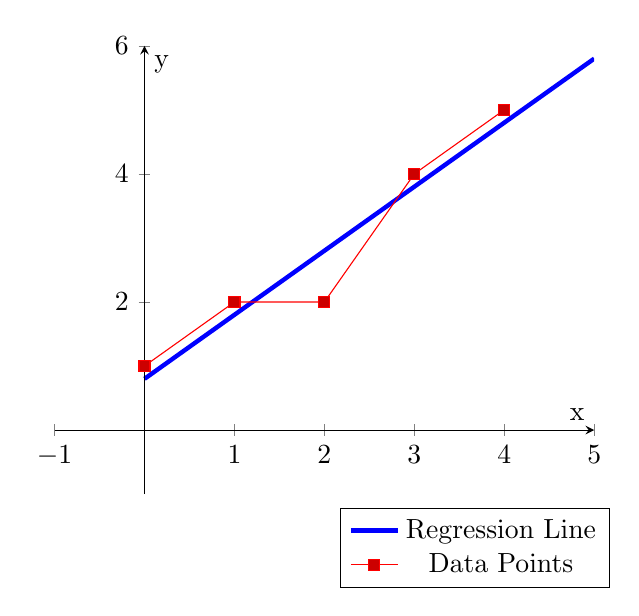
\begin{tikzpicture}
\begin{axis}[
	xlabel=x,
	ylabel=y,
	xmin = -1,
	xmax = 5,
	ymin = -1,
	ymax = 6,
	axis lines = center,
	axis on top = true,
	domain = 0:5,
	legend style = {at={(1.03,-0.03)}},
	%legend style = {legend pos=south east}
	]

	\addplot [mark =none,color=blue, ultra thick] {x + 0.8};
	\addlegendentry{Regression Line}
	\addplot coordinates{
	(0,1)
	(1,2)
	(2,2)
	(3,4)
	(4,5)
	};
	\addlegendentry{Data Points}
\end{axis}
\end{tikzpicture}
\end{center}
\end{solution}

One could clearly do a least squares fit for curves of the form $
y=ax^{2}+bx+c$ in the same way. In this case you want to solve as well as
possible for $a,b,$ and $c$ the system 
\begin{equation*}
\leftB
\begin{array}{ccc}
x_{1}^{2} & x_{1} & 1 \\ 
\vdots & \vdots & \vdots \\ 
x_{n}^{2} & x_{n} & 1
\end{array}
\rightB \leftB 
\begin{array}{c}
a \\ 
b \\ 
c
\end{array}
\rightB =\leftB 
\begin{array}{c}
y_{1} \\ 
\vdots \\ 
y_{n}
\end{array}
\rightB
\end{equation*}
and one would use the same technique as above. Many other similar problems
are important, including many in higher dimensions and they are all solved
the same way.